%%====================================================================%%
%%                      RECURSOS UTILIZADOS                            %%
%%====================================================================%%
\vspace{5mm}
\section{Recursos utilizados}
\label{sec:recursos}

Para o desenvolvimento do sistema foram utilizados recursos de hardware e software responsáveis pela aquisição das variáveis, comunicação através da rede, visualização das informações e atualização remota do firmware. Entre os principais elementos utilizados estão a placa ESP32, o sensor BME280, o protocolo HTTP, a API REST e a plataforma Node-RED.
\vspace{3mm}
\subsection{Descrição do módulo}

O elemento principal de hardware utilizado no projeto foi uma placa baseada no microcontrolador ESP32. A conectividade Wi-Fi disponível no dispositivo foi utilizada para estabelecer a comunicação com os demais elementos do sistema através da rede.

Além do microcontrolador, o módulo utilizado possui um display OLED, empregado durante o desenvolvimento para apresentar localmente algumas informações relacionadas ao funcionamento do sistema. Dessa forma, foi possível observar diretamente no dispositivo os valores adquiridos e algumas informações relacionadas à conexão.

Para aquisição das variáveis ambientais foi utilizado o sensor Bosch BME280. O sensor permite realizar medições de temperatura, umidade relativa e pressão atmosférica, sendo conectado ao ESP32 através do barramento I$^2$C.

A altitude também é apresentada pelo dispositivo, porém esse valor não corresponde a uma medição direta realizada pelo BME280. Seu valor é estimado através da pressão atmosférica medida e de uma pressão de referência ao nível do mar.

Além do BME280, foi utilizado um botão como entrada digital e um LED como saída. O botão permite enviar para o sistema uma informação proveniente de uma entrada física, enquanto o LED permite verificar o funcionamento da comunicação no sentido contrário, uma vez que seu estado pode ser alterado remotamente.

A Figura \ref{fig:pinout-esp} apresenta o diagrama de pinos utilizado como referência durante a implementação.

\begin{figure}[H]
	\centering
	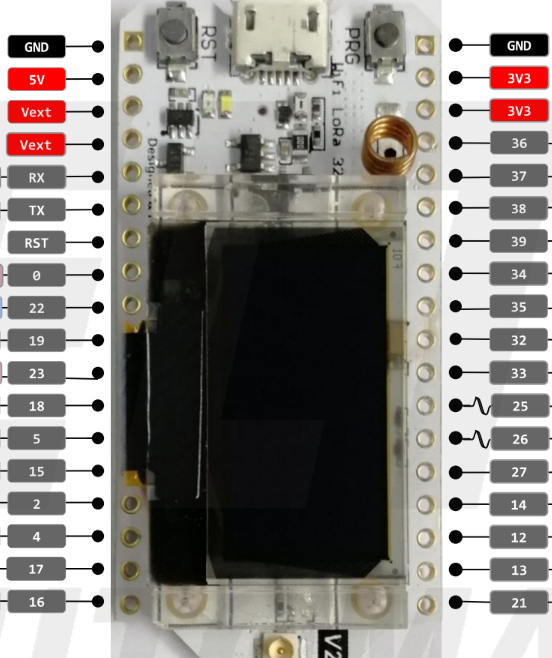
\includegraphics[width=0.3\textwidth, angle=90]{2-imagens/pinout_esp.png}
	\caption{Diagrama de pinos do módulo ESP32 utilizado no projeto.}
	\label{fig:pinout-esp}
\end{figure}


\subsection{Descrição da arquitetura de comunicação}

A arquitetura principal do trabalho foi desenvolvida com o objetivo de permitir a comunicação entre o ESP32 e o Node-RED através de uma API REST utilizando o protocolo HTTP.

O ESP32 é responsável pela aquisição das variáveis físicas. Periodicamente são realizadas leituras do sensor BME280 e do estado do botão. Essas informações são então organizadas pelo firmware e enviadas através da rede.

A API REST é utilizada como meio de comunicação entre os diferentes elementos do sistema. Através de requisições HTTP, os dados adquiridos pelo ESP32 podem ser disponibilizados para o Node-RED, onde são posteriormente tratados e apresentados ao usuário.

De maneira simplificada, o fluxo relacionado à aquisição das informações pode ser representado por:

\begin{center}
	\textbf{BME280 / Botão $\rightarrow$ ESP32 $\rightarrow$ API REST $\rightarrow$ Node-RED}
\end{center}

Além da aquisição, foi implementada uma comunicação no sentido contrário para permitir a atuação remota sobre o LED. Nesse caso, o usuário realiza uma alteração através do dashboard do Node-RED e o comando correspondente é disponibilizado através da API para o ESP32.

O fluxo de atuação pode ser representado por:

\begin{center}
	\textbf{Node-RED $\rightarrow$ API REST $\rightarrow$ ESP32 $\rightarrow$ LED}
\end{center}

Essa estrutura permite demonstrar duas situações diferentes de comunicação. Na primeira, o ESP32 atua como origem das informações adquiridas pelos sensores. Na segunda, o dispositivo recebe uma informação proveniente da interface e realiza uma ação física.

A utilização de uma API REST permite separar a aquisição realizada pelo dispositivo da apresentação realizada no Node-RED. Dessa maneira, a comunicação ocorre através de rotas e mensagens definidas, sem a necessidade de uma ligação direta entre os elementos da interface e cada função implementada no firmware.

\begin{figure}[H]
	\centering
	\resizebox{\linewidth}{!}{%
		\begin{tikzpicture}[
			node distance=1.1cm,
			>=Latex,
			bloco/.style={
				rectangle,
				draw=black,
				rounded corners=3pt,
				minimum width=2.6cm,
				minimum height=1.2cm,
				align=center,
				font=\small
			},
			seta/.style={
				->,
				thick
			}
			]
			
			% --------------------------------------------------------
			% Blocos principais
			% --------------------------------------------------------
			
			\node[bloco] (sensores) {
				\textbf{Aquisição}\\
				BME280 / Botão
			};
			
			\node[bloco, right=of sensores] (esp32) {
				\textbf{ESP32}\\
				Firmware
			};
			
			\node[bloco, right=of esp32] (api) {
				\textbf{API REST}\\
				HTTP
			};
			
			\node[bloco, right=of api] (nodered) {
				\textbf{Node-RED}\\
				Dashboard
			};
			
			
			% --------------------------------------------------------
			% Fluxo de aquisição
			% --------------------------------------------------------
			
			\draw[seta]
			(sensores) --
			node[above, font=\scriptsize] {Leitura}
			(esp32);
			
			\draw[seta]
			(esp32) --
			node[above, font=\scriptsize] {Dados}
			(api);
			
			\draw[seta]
			(api) --
			node[above, font=\scriptsize] {HTTP}
			(nodered);
			
			
			% --------------------------------------------------------
			% LED
			% --------------------------------------------------------
			
			\node[bloco, below=2.2cm of esp32] (led) {
				\textbf{Atuador}\\
				LED
			};
			
			
			% --------------------------------------------------------
			% Fluxo de atuação
			% --------------------------------------------------------
			
			\draw[seta]
			(nodered.south) -- ++(0,-0.8)
			-|
			node[pos=0.25, below, font=\scriptsize] {Comando}
			(api.south);
			
			\draw[seta]
			(api.south) -- ++(0,-1.6)
			-|
			node[pos=0.25, below, font=\scriptsize] {Estado do LED}
			(esp32.south);
			
			\draw[seta]
			(esp32) --
			node[right, font=\scriptsize] {Acionamento}
			(led);
			
			
			% --------------------------------------------------------
			% Identificação dos fluxos
			% --------------------------------------------------------
			
			\node[
			above=0.55cm of api,
			font=\small\bfseries
			] {Fluxo de aquisição};
			
			\node[
			below=2.1cm of api,
			font=\small\bfseries
			] {Fluxo de atuação};
			
		\end{tikzpicture}%
	}
	\caption{Arquitetura principal de comunicação entre o ESP32, a API REST e o Node-RED.}
	\label{fig:arquitetura_principal}
\end{figure}

\subsection{Metodologia de implementação}

A implementação foi realizada inicialmente através do desenvolvimento da comunicação necessária entre o ESP32 e a API REST. O firmware foi preparado para realizar a leitura do sensor BME280 e do botão, além de permitir o acionamento do LED.

Após a leitura correta das variáveis, foi realizada a implementação das requisições HTTP necessárias para a troca de informações. Nessa etapa foram realizados testes para verificar o envio da telemetria e a consulta do estado do atuador.

Em seguida foi desenvolvido o fluxo no Node-RED. A interface passou a consultar as informações disponibilizadas pela API e apresentar os valores de temperatura, umidade e pressão, além dos estados correspondentes ao botão e ao LED.

Posteriormente foi implementado o caminho contrário da comunicação, permitindo que o estado do LED fosse alterado através do dashboard. Dessa forma, foi possível verificar a comunicação tanto no sentido ESP32 para Node-RED quanto no sentido Nodered para ESP32.

Por último, foi configurada a atualização remota do firmware utilizando OTA. Após a programação inicial através da conexão física, foram realizados testes de atualização utilizando a rede Wi-Fi.

Após o funcionamento dos requisitos principais, foram desenvolvidas separadamente algumas funcionalidades adicionais, apresentadas posteriormente na subseção de desenvolvimento extra.


